
%\documentclass[12pt]{report}

\documentclass[12pt]{article}
%\usepackage{natbib}  % used for citations
\usepackage[parfill]{parskip} %used for formatting style of text



\usepackage{graphicx,fancyhdr}
\usepackage{amssymb,amsmath}
\usepackage{epigraph,fancyvrb,eqparbox}
\usepackage[multiple]{footmisc}
\usepackage{menukeys}
\usepackage{menukeys}
\usepackage{url}
\usepackage[colorlinks = true, linkcolor = blue, urlcolor = blue]{hyperref}
\usepackage{setspace}

\pagestyle{fancyplain}

%\usepackage{hyperref}
%\usepackage{epsf,psfig,graphicx,fancyheadings}
% \textwidth 7in
% \textheight 9in
% \oddsidemargin 0in
% \topmargin -.25in

%-----------------------------------------------
% The following settings are from Dr. Davidian's
% ST810A Handout on Advanced LaTeX Features

%\setlength{\paperheight}{11.0in}
%\setlength{\paperwidth}{8.5in}

%%%%%%%%%%%%%%%%%%%%%%%%%%%%%%%%%%%%%%%%%%%%%%%%%
% For Desktop @ CalPoly (for Postscript)

%\setlength{\oddsidemargin}{0.5in}
%\setlength{\evensidemargin}{0.5in}
%\setlength{\topmargin}{-.5in}

%%%%%%%%%%%%%%%%%%%%%%%%%%%%%%%%%%%%%%%%%%%%%%%%%
% For Laptop @ Calpoly (for Postscript)

% \setlength{\oddsidemargin}{0.in}
% \setlength{\evensidemargin}{0.in}
% \setlength{\topmargin}{0.25in}

%%%%%%%%%%%%%%%%%%%%%%%%%%%%%%%%%%%%%%%%%%%%%%%%%
% For Desktop @ CalPoly (for PDF)

%\setlength{\oddsidemargin}{0.in}
%\setlength{\evensidemargin}{0.in}
%\setlength{\topmargin}{-.5in}
%
%%%%%%%%%%%%%%%%%%%%%%%%%%%%%%%%%%%%%%%%%%%%%%%%%%
%% For Laptop @ Calpoly (for PDF)
%
%% \setlength{\oddsidemargin}{0.in}
%% \setlength{\evensidemargin}{0.in}
%% \setlength{\topmargin}{0.25in}
%
%
%
%\setlength{\oddsidemargin}{0.0in}
%\setlength{\topmargin}{-0.5in}
%\setlength{\headheight}{0.20in}
%\setlength{\headsep}{3ex}
%\setlength{\baselineskip}{2ex}
%\setlength{\textheight}{9in}
%\setlength{\textwidth}{6.4in}
%\renewcommand{\baselinestretch}{1.1}

% Sets margins to 1 in
\addtolength{\oddsidemargin}{-.5in}%
\addtolength{\evensidemargin}{-.5in}%
\addtolength{\textwidth}{1in}%
\addtolength{\textheight}{1.3in}%
\addtolength{\topmargin}{-.8in}%

%\setlength{\headheight}{0.20in}
%\setlength{\headsep}{3ex}
%\setlength{\headrulewidth}{0.2pt}
%\setlength{\footrulewidth}{0.15pt}
%\setlength{\parskip}{2.3ex}
% %set to no indentation
%\setlength{\parindent}{0.0in}
%\setlength{\baselineskip}{2ex}
%\setlength{\textheight}{9.in}
%\setlength{\textwidth}{6.5in}

\def \doublespace{\openup 2\jot}
% For double or 1.5 spacing
%\renewcommand{\baselinestretch}{1.5}
\tolerance=500

\def\boxit#1{\vbox{\hrule\hbox{\vrule\kern6pt
\vbox{\kern6pt#1\kern6pt}\kern6pt\vrule}\hrule}}
\renewcommand{\theequation}{\thesection.\arabic{equation}}
% The following for TOC
%\renewcommand{\thepage}{\roman{page}}
% to be followed by this for the main text
\renewcommand{\thepage}{\arabic{page}}


%-----------------------------------------------

%%%%%%%%%%%%%%%%%%%%%%%%%%%%%%%%%%%%%%
%Define any shortcut aliases below

\newtheorem{theo}{Theorem}[section]

\newenvironment{note}{\begin{quote}\emph{Note:\ }}{\end{quote}}
\newenvironment{defn}{
\begin{description}
\item[Definition ]}
{\end{description}}

\newenvironment{ttscript}[1]{%
    \begin{list}{}{%
    \settowidth{\labelwidth}{\texttt{#1}}
    \setlength{\leftmargin}{\labelwidth}
    \addtolength{\leftmargin}{\labelsep}
    \setlength{\parsep}{0.5ex plus0.2ex minus0.2ex}
    \setlength{\itemsep}{0.3ex}
    \renewcommand{\makelabel}[1]{\texttt{##1\hfill}}}}
    {\end{list}}

\newcommand{\bt}{\begin{tabular}}
\newcommand{\et}{\end{tabular}}
\newcommand{\bc}{\begin{center}}
\newcommand{\ec}{\end{center}}
\newcommand{\bi}{\begin{itemize}}
\newcommand{\ei}{\end{itemize}}
\newcommand{\be}{\begin{enumerate}}
\newcommand{\ee}{\end{enumerate}}
\newcommand{\bq}{\begin{quote}}
\newcommand{\eq}{\end{quote}}
\newcommand{\vect}[1]{\mbox{\boldmath $ #1$}}
\newcommand{\avg}[1]{$\overline{#1}$}
\newcommand{\bmp}{\begin{minipage}}
\newcommand{\emp}{\end{minipage}}
\newcommand{\hr}{\u{\hspace{7in}}}
\newcommand{\sr}{\u{\hspace{5in}}}
\newcommand{\chs}{\chi^2}

\newcommand{\labn}[1]{\Large{\textbf{\fbox{Lab #1}}}\hspace{0.1in} \normalsize{\emph{Some of these problems may be more challenging than others. Please feel free to work with others, attend office hours, or post on the course discussion forum if you need help.  While collaboration with other students is encouraged, each student is responsible for submitting his or her own work.  This assignment should be submitted in one well-commented SAS program.  For any questions that require a written answer, do so in the SAS comments.  Be sure to re-name the uploaded SAS scripts according to the naming convention}} \texttt{LastnameFirstinitial\textunderscore Lab\#.sas} (\emph{e.g.,} \texttt{PileggiS\textunderscore Lab#1.sas}).}


\newcommand{\hd}[1]{\lhead{STAT 330/530: Lab #1}\rhead{Pileggi, FA17}}
\newcommand{\bs}{\underline{\hspace{0.5in}}}

%\newcommand{\bv}{\footnotesize
%\bmp{.5\textwidth}
%\begin{Verbatim}[frame=single,label=SAS Code,commandchars=\\\{\}],xrightmargin=.5\textwidth}
%
%\newcommand{\ev}{\end{Verbatim}
%\emp
%\normalsize}

\newcommand{\bv}{\begin{code}}
\newcommand{\ev}{\end{code}}

 \newenvironment{code}[1]%
  {\vspace{.1in}\footnotesize\Verbatim[frame=single,label=SAS Code,commandchars=\\\{\},xrightmargin=#1\textwidth,framesep=.2in,labelposition=all]}
  {\endVerbatim\normalsize}

\newenvironment{craw}[2]%
{\vspace{.1in}\footnotesize\Verbatim[frame=single,label=#2,commandchars=\\\{\},xrightmargin=#1\textwidth,framesep=.2in,labelposition=all]}
  {\endVerbatim\normalsize}

\newenvironment{cbox}[1]%
{\vspace{.1in}\footnotesize\Verbatim[frame=single,commandchars=\\\{\},xrightmargin=#1\textwidth,framesep=.2in,labelposition=all]}
  {\endVerbatim\normalsize}

\newcommand{\head}[1]{\large \textbf{#1} \normalsize}

\newcommand{\ttt}[1]{\textbf{\texttt{#1}}}


\newcommand{\bsval}[1]{\underline{\hspace{0.2in}{[#1]}\hspace{0.2in}}}

\newcommand{\ttb}{\textbf}
\newcommand{\tte}{\emph}
\newcommand{\ttu}{\underline}



\newcommand{\jdhr}{\vspace{0.2in}\hrule}


\newcommand{\uspace}[1]{\underline{\hspace{#1}}}

\newenvironment{ident}{\begin{list}{}{}
         \item[]}{\end{list}}

\newenvironment{proposition}{
\begin{description}
\item[Proposition: ]}
{\end{description}}

\newcommand{\bpr}{\begin{proposition}}
\newcommand{\epr}{\end{proposition}}



% \newenvironment{example}
%     {
%         \begin{list}{\textbf{Example:}}
%         {
%         \settowidth{\labelwidth}{}
%         \setlength{\leftmargin}{\labelwidth}
%         }
%     }
%     {\end{list}}


\newenvironment{example}{
\jdhr \vspace{-.17in}\jdhr
\textbf{Example: }}
{}

\newcommand{\bex}{\begin{example}}
\newcommand{\eex}{\end{example}}

\newenvironment{onyourown}{
\jdhr \vspace{-.17in}\jdhr
\textbf{On Your Own: }}
{}

\newcommand{\boy}{\begin{onyourown}}
\newcommand{\eoy}{\end{onyourown}}


%\newenvironment{debug}{
%\jdhr \vspace{-.17in}\jdhr
%\ttb{Debug the Code}
%\fbox{
%\bmp{.95in}
%\includegraphics[height=.35in]{C:/images/bug4.jpg}\includegraphics[height=.35in]{C:/images/buggy8.jpg}
%\emp}
%}
%{\jdhr}

\newenvironment{debug}{
\jdhr \vspace{-.17in}\jdhr
\ttb{Debug the Code: }
\fbox{
\bmp{.95in}
\includegraphics[height=.35in]{C:/images/bug4.jpg}\includegraphics[height=.35in]{C:/images/mushi90.jpg}
\emp}
}
{}


\newcommand{\bbug}{\begin{debug}}
\newcommand{\ebug}{\end{debug}}


\begingroup
  \catcode `_=11
  \gdef\myuscore{_}
  \catcode `~=11
  \gdef\mytilde{~}
  \catcode `\|=0
  \catcode `\\=11
  |gdef|mybs{\}
|endgroup

%Define any shortcut aliases above


%....................................................................
%....................................................................
%....................................................................
%....................................................................
%....................................................................
%....................................................................
%....................................................................
%....................................................................



\usepackage{amssymb}
				

\begin{document}
\hd{12}
\labn{12}
\vskip10pt
This US Surgeon General's warning was placed on the side of cigarette packages beginning in 1985.   Prior to the placement of the warning, studies had to be conducted to investigate the effects of smoking during pregnancy.  The data provided are part of the Child Health and Development Studies, which was a comprehensive investigation of all pregnancies that occurred between 1960 and 1967 among women in the Kaiser Foundation Health Plan in the San Francisco-East Bay area.  Despite the warnings which went into effect in 1985, the National Center for Health Statistics found that 15\% of women who gave birth in 1996 smoked during their pregnancy.  (What year were you born?)
\\\\
%\vskip5pt
Why do we care about baby birth weight?  Birth weight is a measure of a baby's maturity.  Typically, smaller babies have lower survival rates than than larger babies.  In this study, the rate at which babies died within 28 days of birth was 150 per thousand births for low birth weight babies, compared to 5 per thousand for babies of 'normal' weight.  Babies that weigh under 5.5 pounds are considered of low birth weight.
\\\\
%\vskip5pt
\texttt{babies.csv}
\\\\
%\vskip5pt
\begin{tabular}{r|l}
\ttt{bwt} & baby's weight at birth in ounces\\
\ttt{gestation} & length of pregnancy in days\\
\ttt{parity} & 0=first born, 1=otherwise\\
\ttt{age} & mother's age in years\\
\ttt{height} & mother's height in inches\\
\ttt{weight} & mother's pregnancy weight in pounds\\
\ttt{smoke} & smoking status of mother: 0=not now, 1=yes now\\
\end{tabular}

\begin{enumerate}
\item Assign the computer location of your STAT 330 data set to a macro variable called \ttt{path}.
\item Read the \ttt{babies.csv} data into SAS using your \ttt{path} macro variable.  Write a couple of procedures to familiarize yourself with the data.
\end{enumerate}
\emph{Follow the subsequent steps to export summary statistics used to investigate the relationship between mother's smoking status and baby birth weight.}
\begin{enumerate}
\setcounter{enumi}{2}
\item Use one SAS procedure to obtain the sample size, minimum, maximum, sample mean, and sample standard deviation of baby birth weight separately for smoking and non-smoking mothers.  Based on your descriptive statistics, does there appear to be a relationship between mother's smoking status and baby birth weight? Note your observations in a comment in your SAS code.  Your summary statistics should appear as shown below.
\item[] 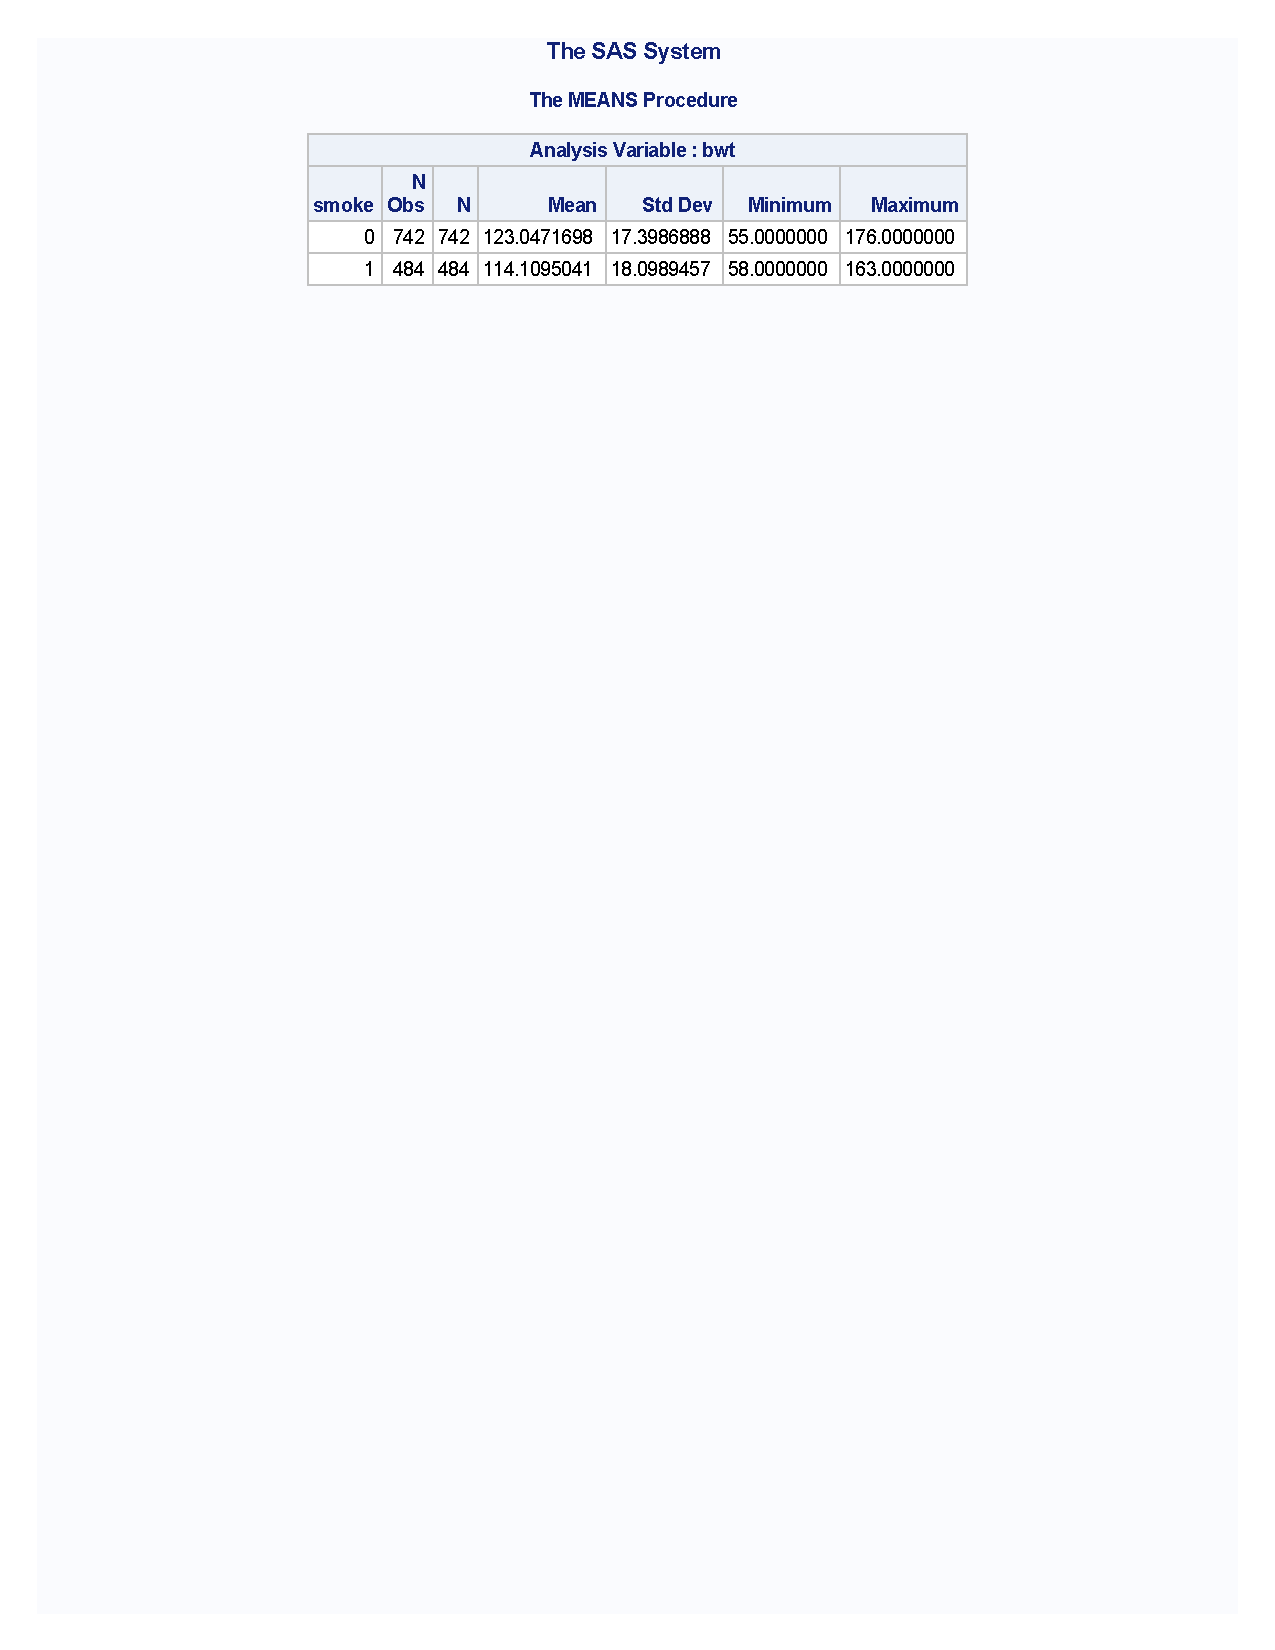
\includegraphics[trim=5cm 22cm 5cm 2.0cm,clip]{q3_stats.pdf}
\item Modify your code from the previous question to create a SAS data set with the summary statistics.  Print this data set - your results should match those shown below.
\item[] 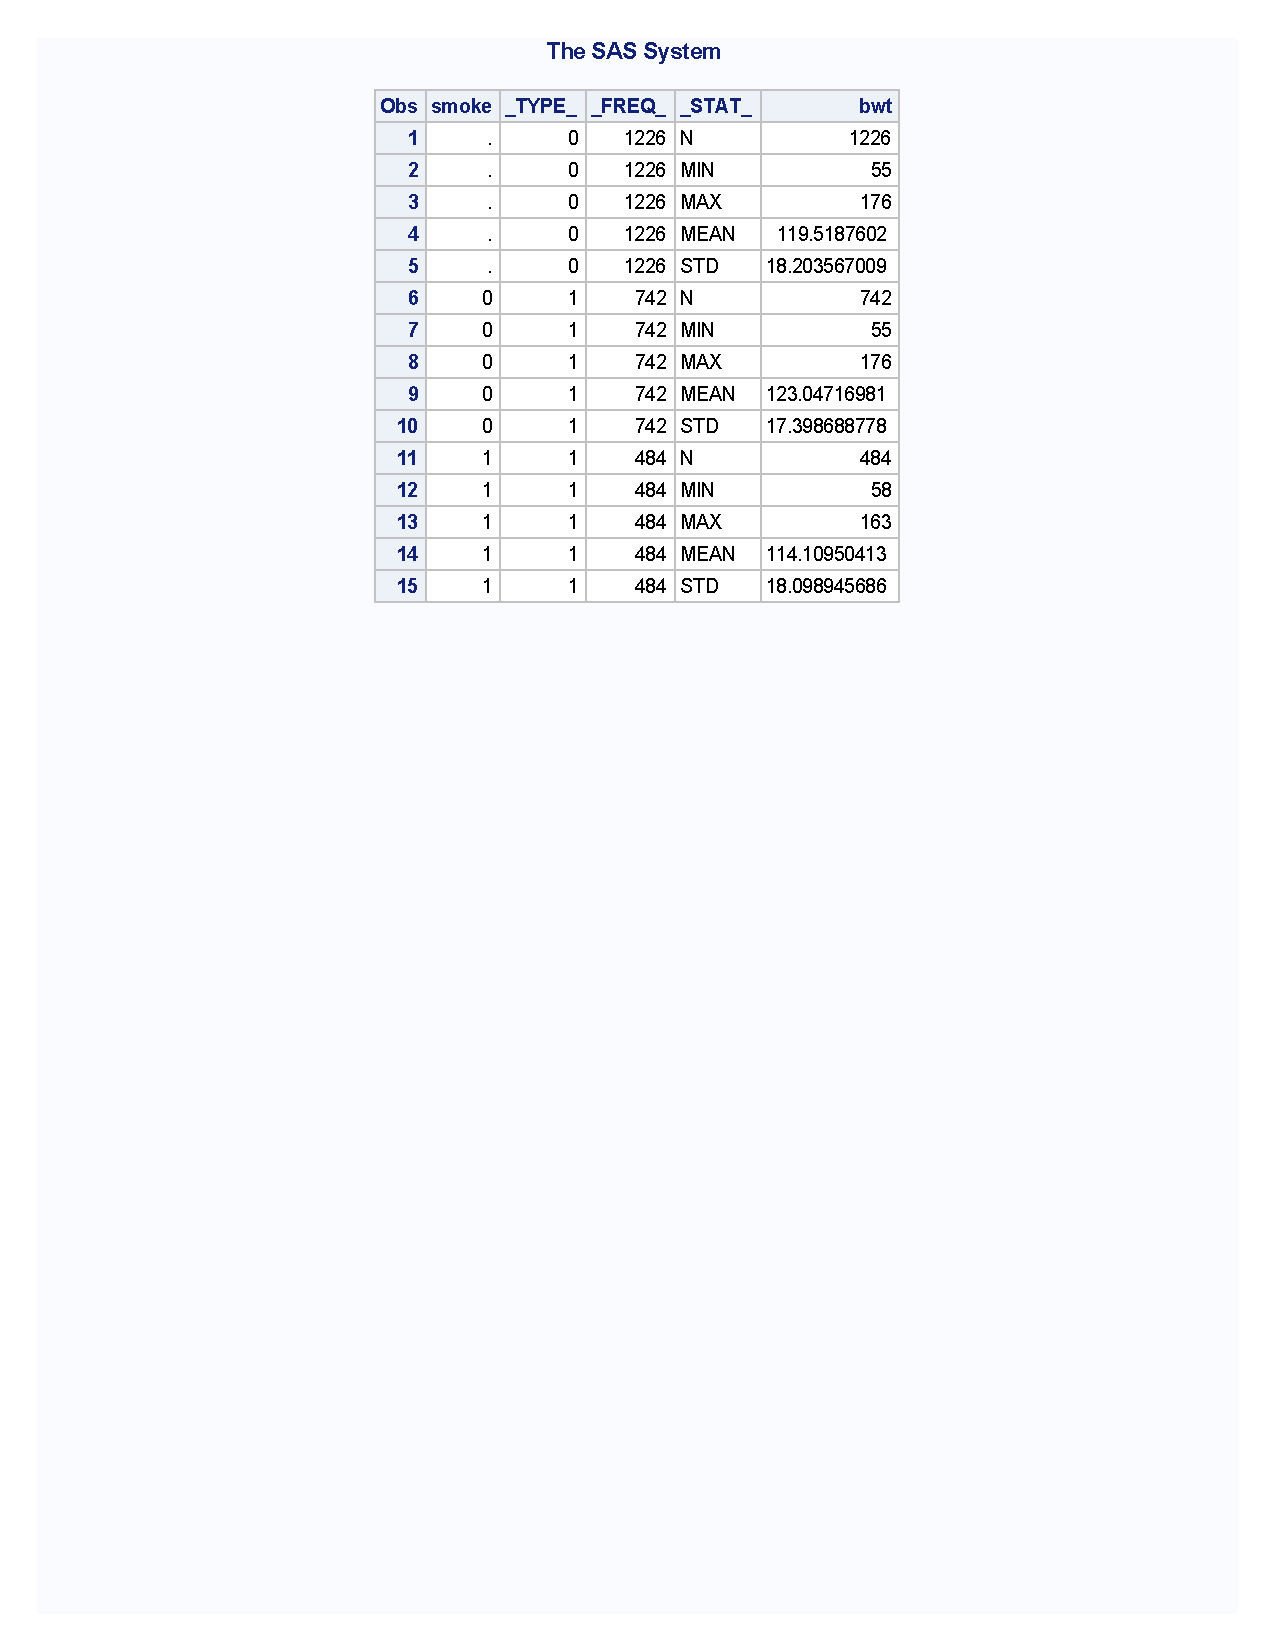
\includegraphics[trim=5cm 17cm 5cm 1.5cm,clip]{q3_statsout.pdf}
\item Rearrange the summary statistics data such that the columns correspond to the statistics and the rows correspond to mother smoking status.  Note that a period (.) indicates the overall summary statistics, regardless of mother's smoking status.  \underline{Exclude} the overall summary statistics when you re-arrange the data.  Your summary statistics data should appear as shown below.
\item[] 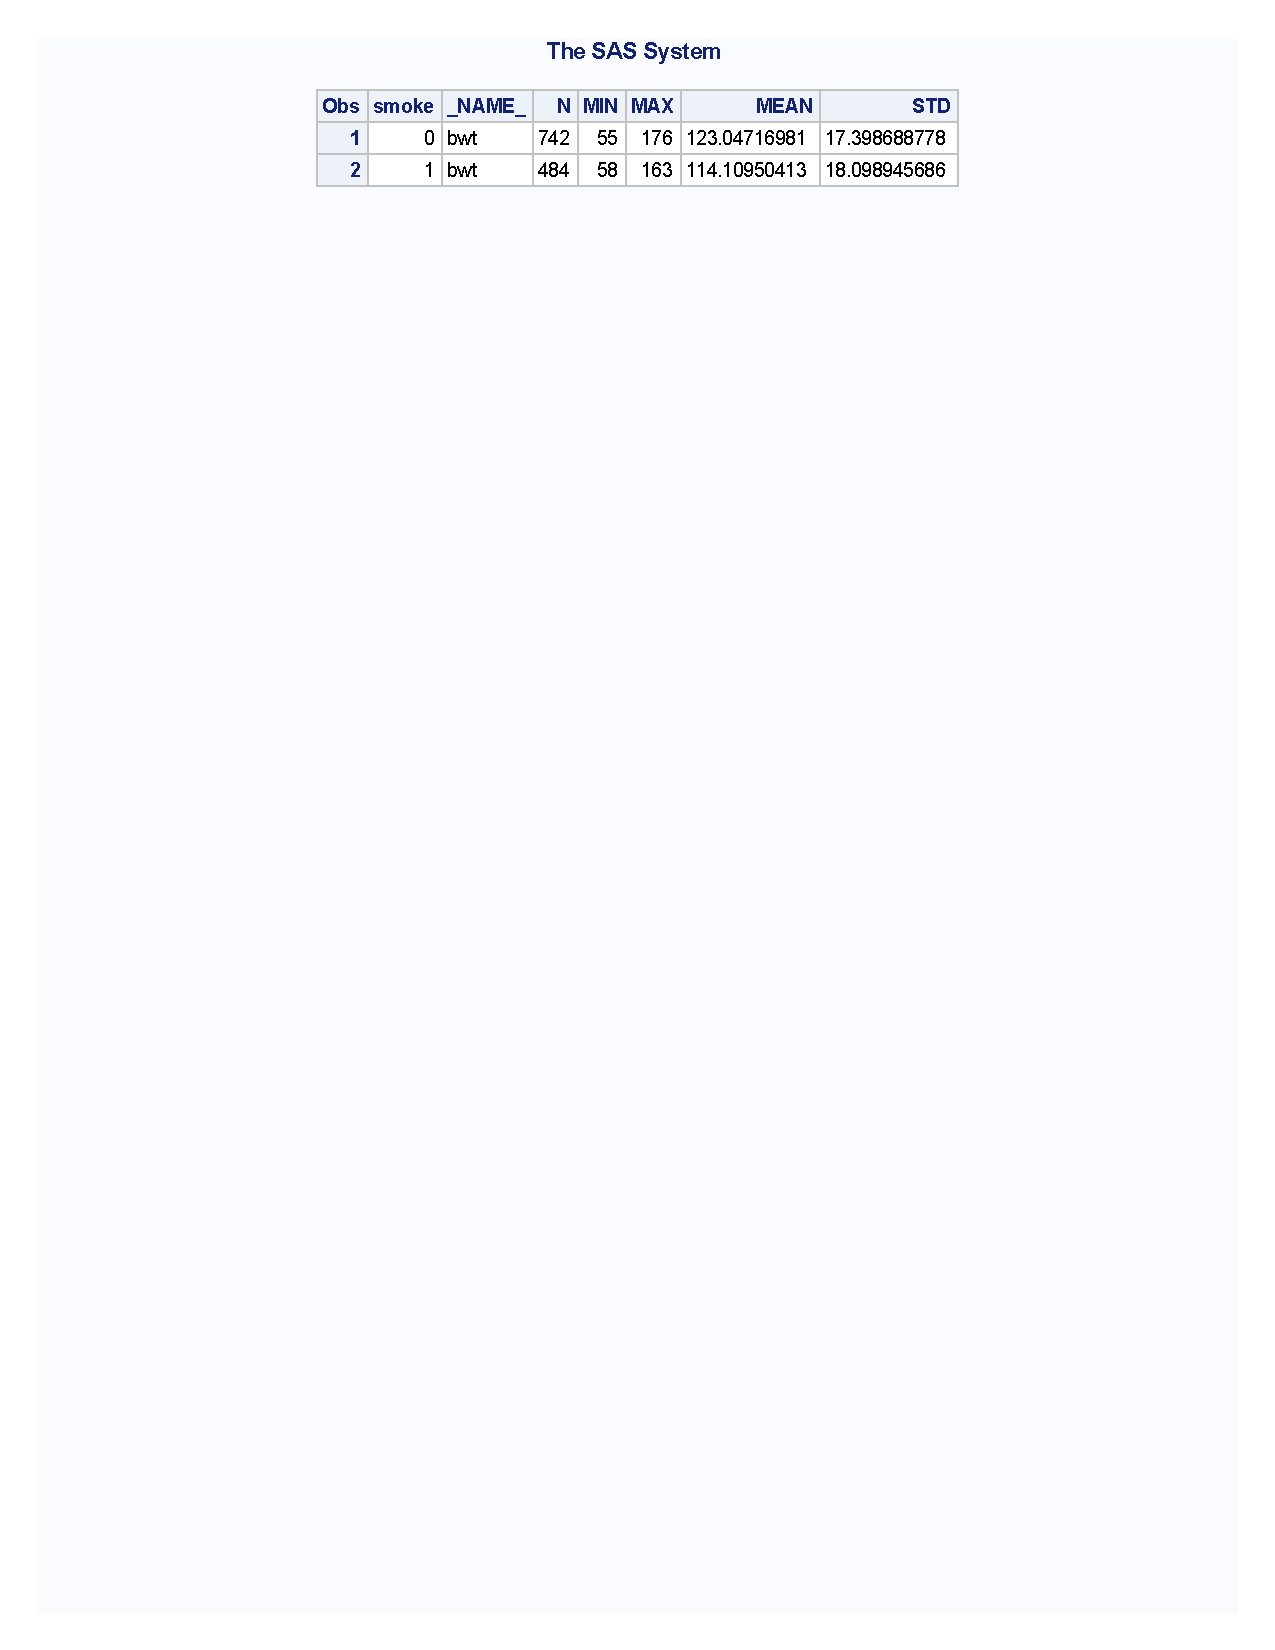
\includegraphics[trim=5cm 24cm 5cm 1.5cm,clip]{q3_statstrans.pdf}
\item Modify the summary statistics data.
\begin{enumerate}
\item Make sure that all means and standard deviations are formatted to one decimal place.
\item Create and apply a format such that 0 displays as ``Non-smoking mothers'' and 1 displays as ``Smoking mothers''.
\item Only retain relevant variables/observations.
\end{enumerate}
\item[] Your final summary statistics data set should appear as:
\item[] 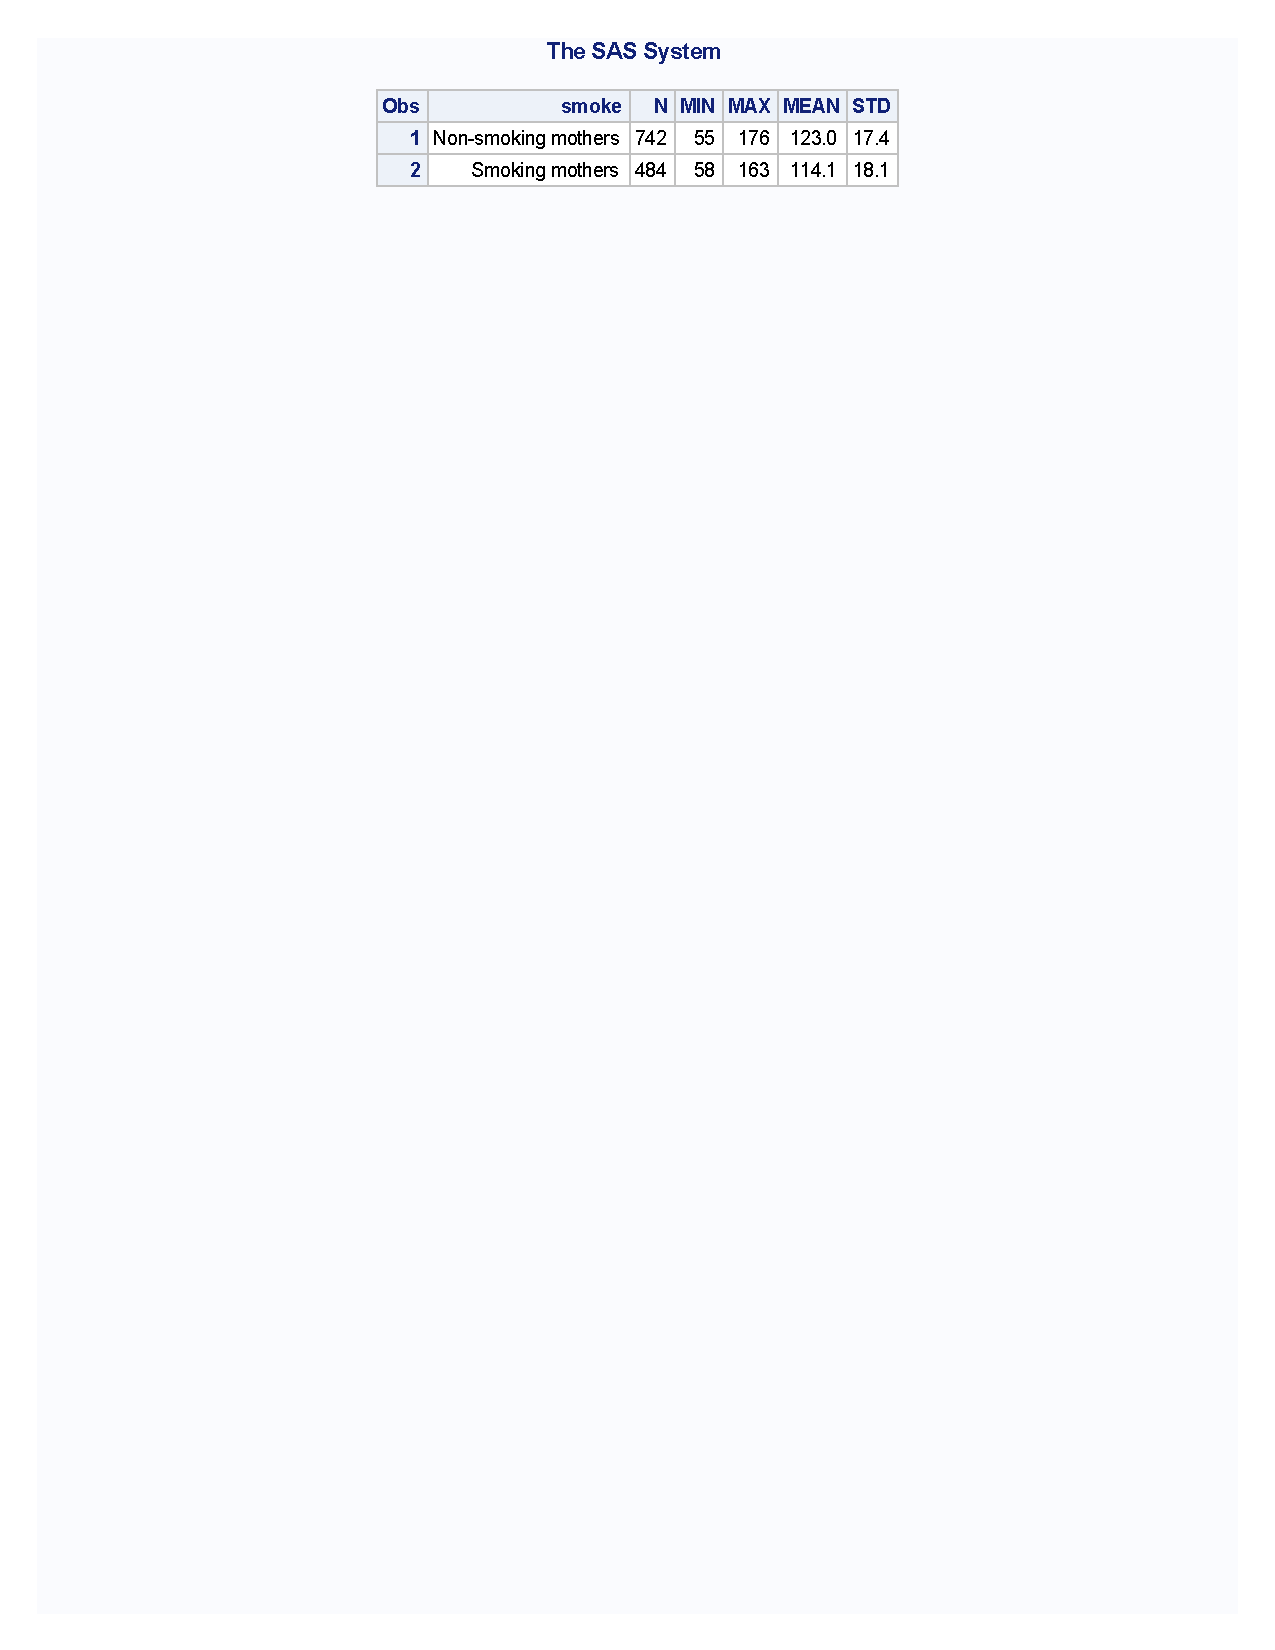
\includegraphics[trim=5cm 24cm 5cm 1.5cm,clip]{q6_statsfinal.pdf}
\item Export the summary statistics data to \ttt{BabiesSummaryStats.csv} using the \ttt{path} macro variable.  Open the \ttt{BabiesSummaryStats.csv} file and verify that everything appears as intended.  Upload the \ttt{BabiesSummaryStats.csv} file to PolyLearn in addition to your SAS program.
\end{enumerate}
\emph{At some point in your career, it may be necessary to create a succinct table of essential statistical results.  Follow the subsequent steps to get essential output from a two-sample t-test.}
\begin{enumerate}
\setcounter{enumi}{7}
\item Perform a two-sample t-test to determine if we have evidence of a difference in population mean birth weight among babies born to smoking and non-smoking mothers.
\item Modify your code from the previous question to create two SAS data sets - one that contains the hypothesis test results and one that contains the confidence interval results.  Your data sets should appear as those shown below.
\item[] 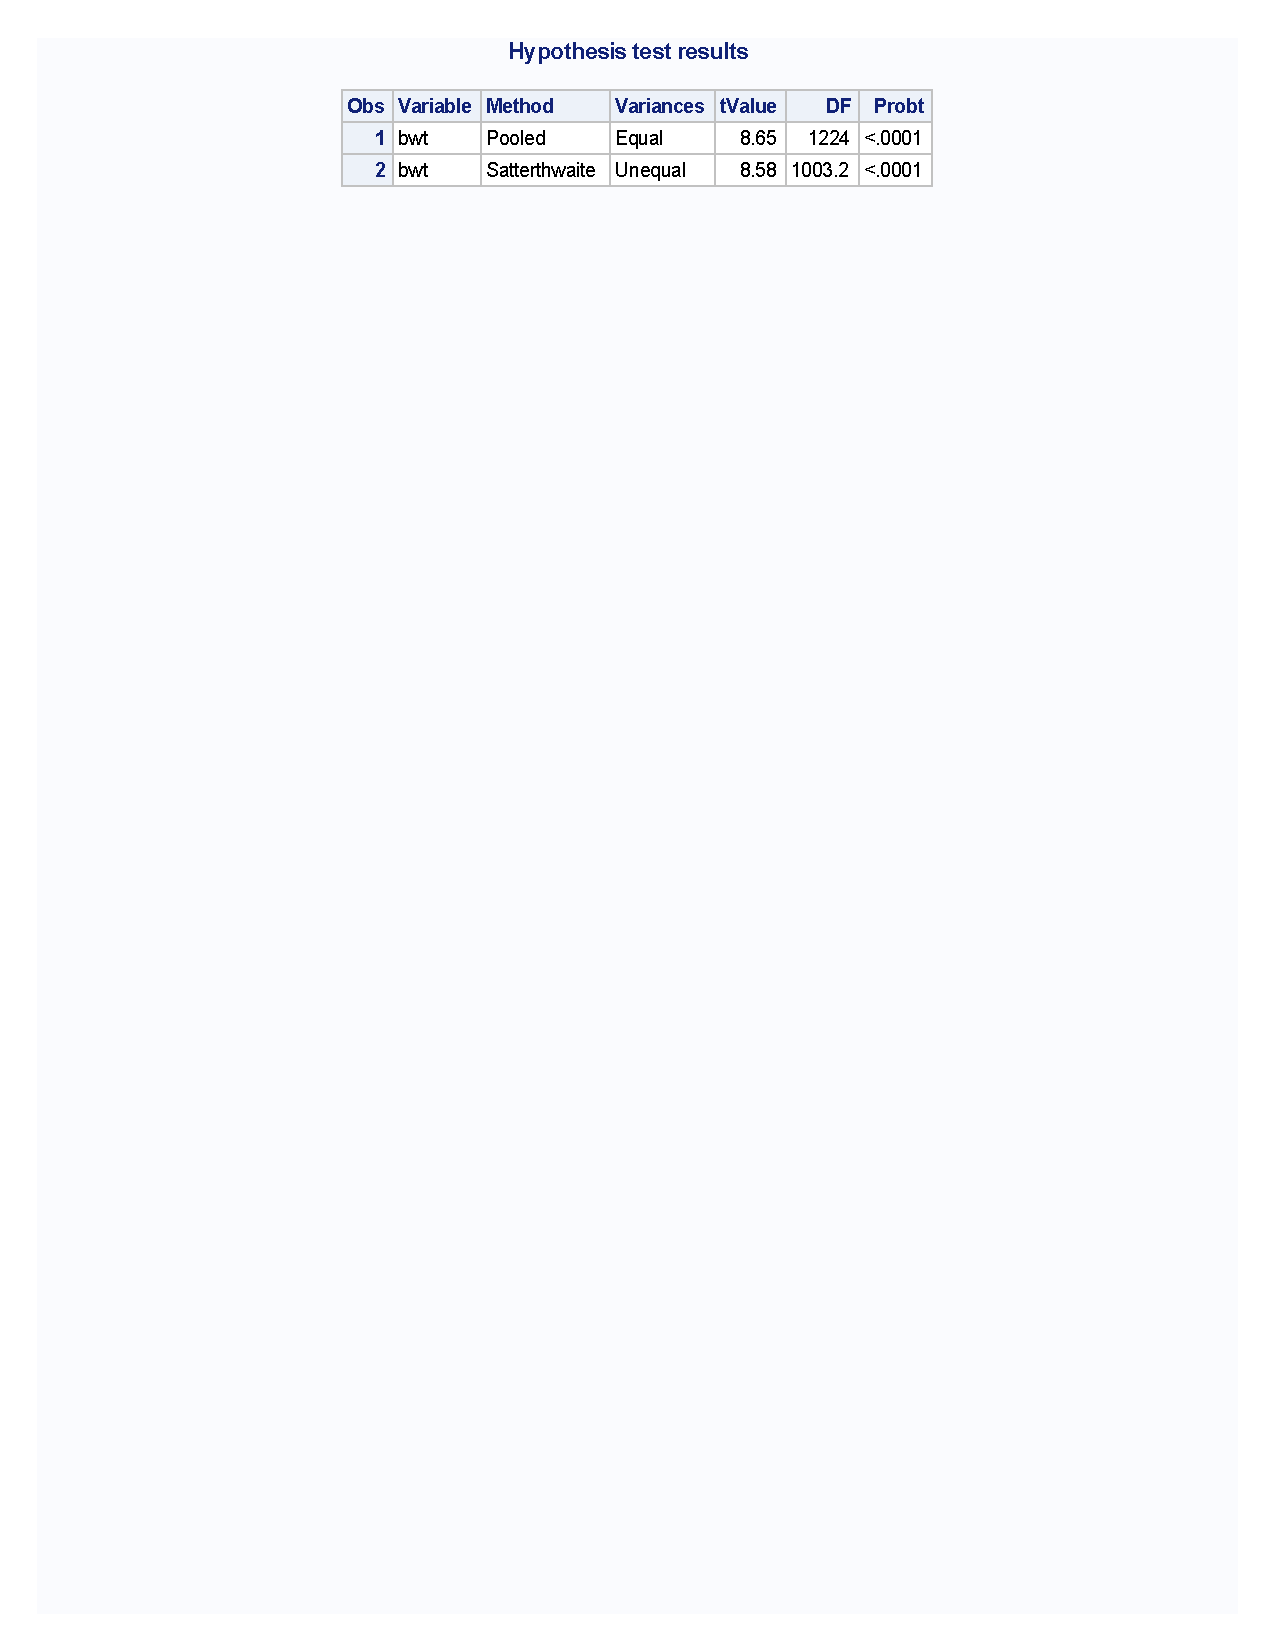
\includegraphics[trim=3cm 24cm 3cm 0.5cm,clip]{q9_ht.pdf}
\item[] 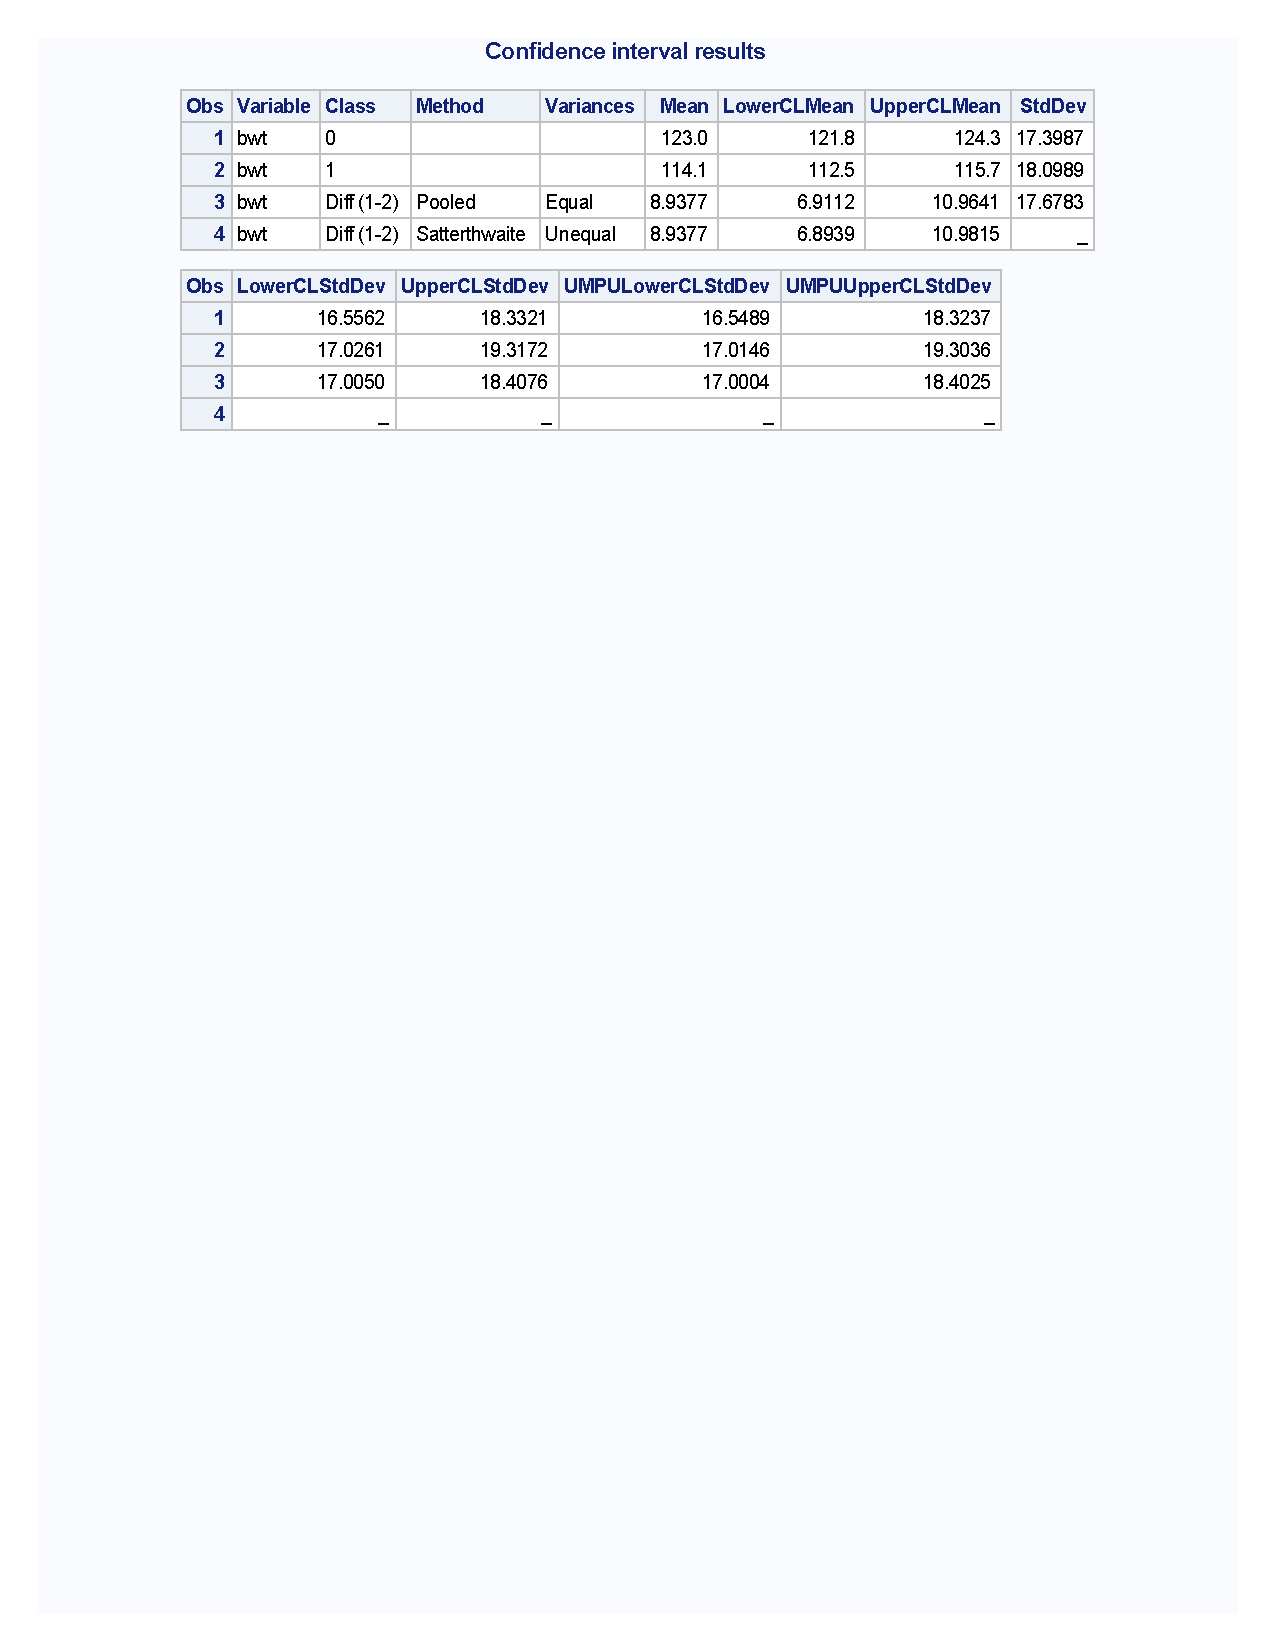
\includegraphics[trim=3cm 20cm 3cm 0.5cm,clip]{q9_ci.pdf}
\item Combine these two data sets such that you only keep results for the equal variances method.  From the hypothesis test results, keep the degrees of freedom, test statistic, and p-value.  From the confidence interval results, keep the lower and upper confidence interval limits.  Print this data set - it should appear as shown below.
\item[] 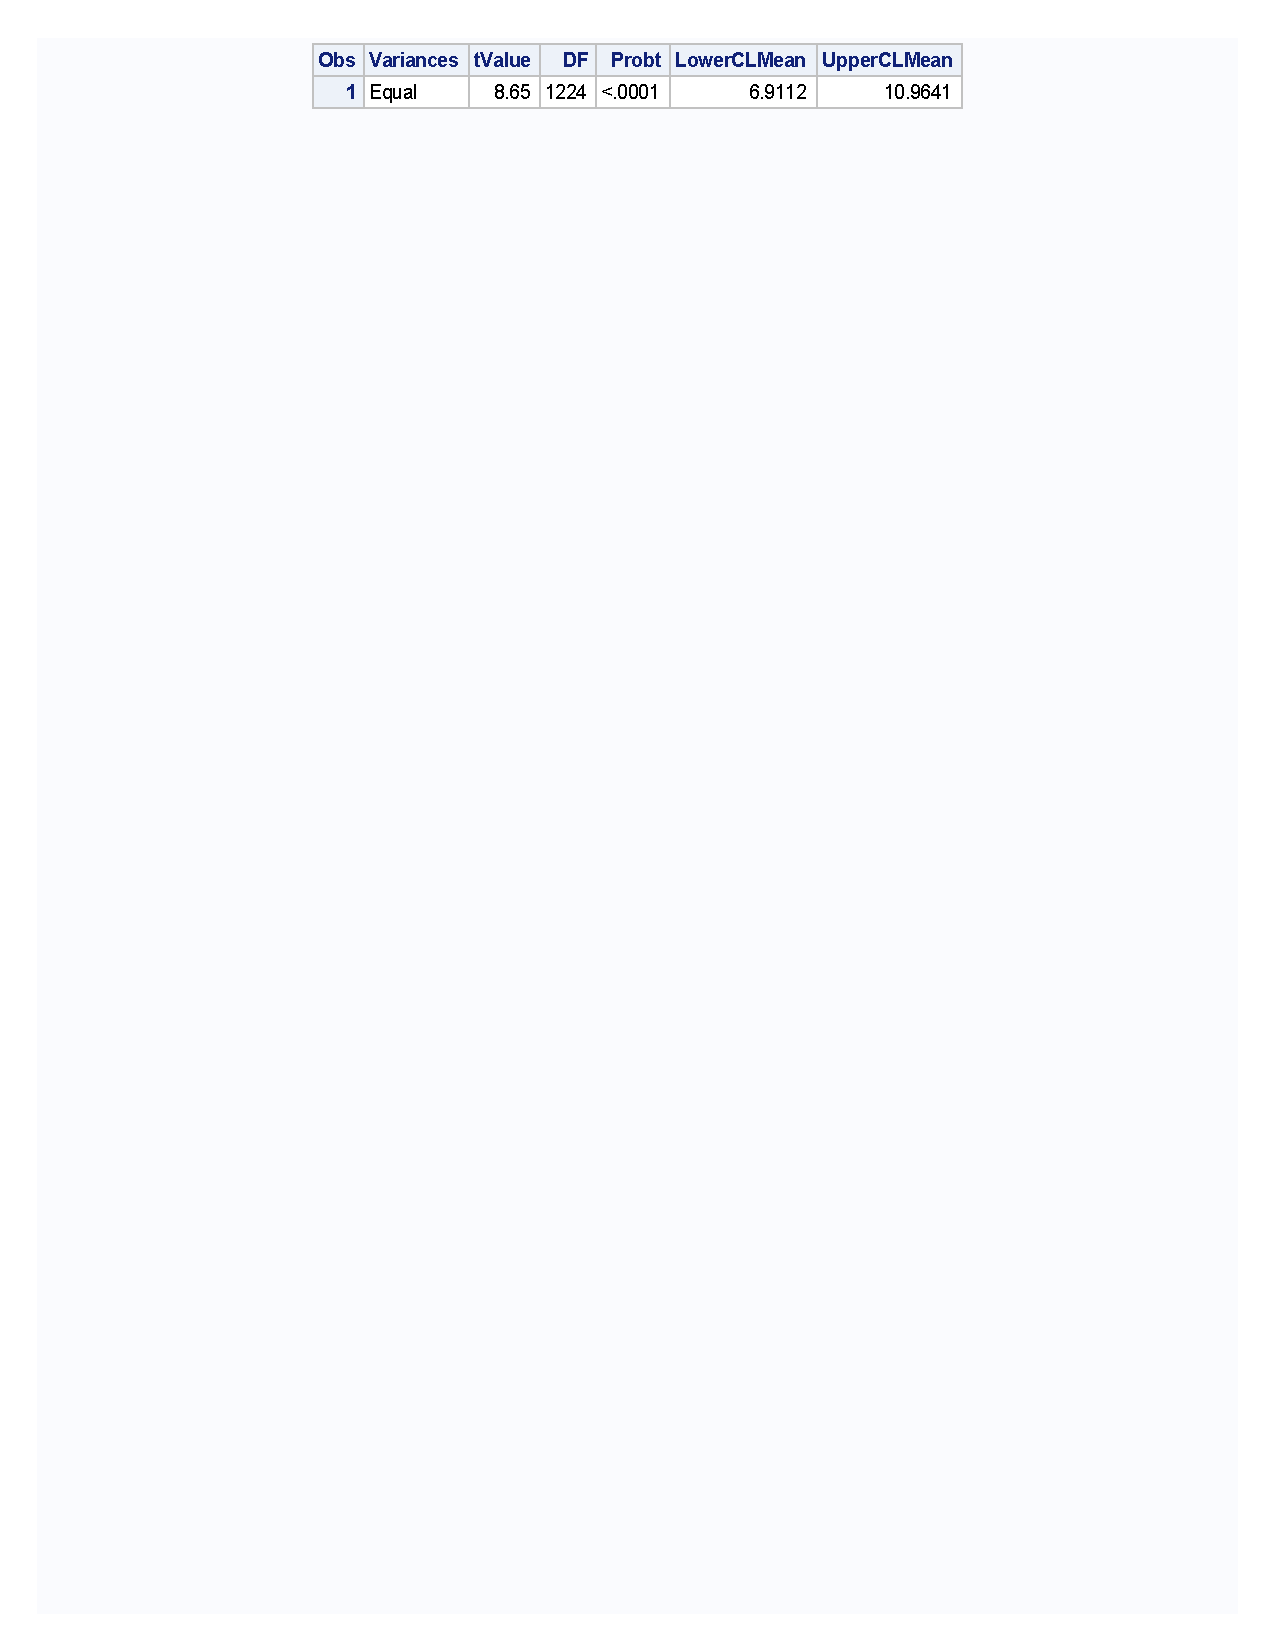
\includegraphics[trim=3cm 25cm 3cm 0.5cm,clip]{q10_combined.pdf}
\item In a comment in your SAS code, provide a brief interpretation of these results.
\end{enumerate}
%\item Follow the subsequent steps to fit a linear regression model, explore results, and export residual values.  It may be helpful to refer to Lecture 10 notes.
%\begin{enumerate}
%\item Fit a linear regression model with baby's birth weight as the dependent variables and all other variables in  the data set as the independent variables.
%\item Examine the parameter estimates.
%\begin{enumerate}
%\item Are all variables associated with baby's birth weight at the 0.05 significance level?  Note your findings in a comment in your SAS code.
%\item Which variables appear to be associated with having a baby with \emph{lower} birth weight?  Explain your findings in a comment in your SAS code.
%\end{enumerate}
%\item Modify your code from (a) to create a SAS data set with the observations' predicted values and residuals based on the regression model.
%\item Sort this SAS data set based on the value of the residual.
%\item Use a SAS procedure to determine how many babies had predicted birth weights that differed from observed birth weights by more than 50 ounces (that is 3.125 pounds!)  Note your findings in a comment in your SAS code.
%\item Export the data set with the regression model's predicted values and residuals to a csv file called \ttt{BabiesResids.csv} using the \ttt{path} macro variable.  Open the \ttt{BabiesResids.csv} file and verify that everything appears as intended.
%\end{enumerate}


\end{document} 